\section{Background}

\begin{frame}{}
  \begin{center}
    \Large{Why is this not about ANNS anymore?}
  \end{center}
\end{frame}

\begin{frame}{}
  \begin{definition}[Random Sampling without Replacement]
    Given a data set \(X\), we uniformly pick \(k\) elements
    from \(X\) such that none repeat.
  \end{definition}

  \vspace{2em}

  Seems simple enough, why care?
\end{frame}

\begin{frame}{Baseline (\(O(n^2)\) worst case)}
  \begin{algorithm}[H]
  \caption{Naive Pick and Remove}
  \begin{algorithmic}
    \Input{Data set \(X\)}
    \Output{Sample \(S\) with \(|S| = k\)}
    \For{\(i = 1..k\)}
      \State{Pick \(x\) u.a.r. from \(X\)}
      \State{Add \(x\) to \(S\)}
      \State{Remove \(x\) from \(X\)}
    \EndFor
    \State{\Return{\(S\)}}
  \end{algorithmic}
  \end{algorithm}
\end{frame}

\begin{frame}{Improvement: Priority Sampling (\(\O(n)\) w.h.p.
  \footnote{Probability at least \(1 - \O(n^{-c})\) for some
  \(c > 0\)})}
  \begin{algorithm}[H]
  \caption{Priority Sampling via Quick Select}
  \begin{algorithmic}
    \Input{Data set \(X\), Sample size \(k\)}
    \Output{Sample with size \(k\)}

    \State{Assign priority from \(\Unif(0, 1)\) to each element
    of \(X\)}
    \State{\Return{\textsc{QuickSelect(\(X, k\))} by priority}}
  \end{algorithmic}
  \end{algorithm}
\end{frame}

\begin{frame}{Recap: \textsc{QuickSelect}}
  \begin{algorithm}[H]
  \caption{Quick Select}
  \begin{algorithmic}
    \Input{Data set \(Y\), Sample size \(l\)}
    \Output{Sample with size \(l\)}

    \State{Pick \(p\) u.a.r. from \(Y\)}
    \State{\(LE \gets \{y \in Y : y \leq p\}\)}
    \State{\(G \gets \{y \in Y : y > p\}\)}

    \IIf{\(|LE| = k\)}{\Return{\(LE\)}}
    \IElsIf{\(|LE| > k\)}{\Return{\textsc{QuickSelect(\(LE, l\))}}}
    \IElse{\Return{\textsc{Concat(\(LE\), QuickSelect(\(G,
    l - |LE|\)))}}}
  \end{algorithmic}
  \end{algorithm}
\end{frame}

\begin{frame}{Alternate Improvement: Permutation (\(\Theta(n)\))}
  \begin{algorithm}[H]
  \caption{Permutation Sampling}
  \begin{algorithmic}
    \Input{Data set \(X\), Sample size \(k\)}
    \Output{Sample with size \(k\)}

    \State{Generate swapping locations \(H\) such that 
    \(i \leq H[i] < n\)}
    \State{\textsc{Shuffle(\(X, H\))}}
    \State{\Return{\(X[{}:k]\)}}
  \end{algorithmic}
  \end{algorithm}
\end{frame}

\begin{frame}{Recap: Shuffle}
  \begin{algorithm}[H]
  \caption{Shuffling via Fisher-Yates}
  \begin{algorithmic}
    \Input{Array \(A\), Pre-generated swap targets \(H\)}

    \For{\(i = 1, 2, \ldots, n\)}
      \State{\textsc{Swap(\(A[i], A[H[i]]\))}}
    \EndFor
  \end{algorithmic}
  \end{algorithm}
\end{frame}

\begin{frame}{Problem Statement}
  \begin{center}
    Observation: Existing algorithms run proportional to \(n\),
    not \(k\).
  \end{center}

  Is this a problem?
  \begin{itemize}
    \item When \(k \sim \Theta(n)\), no.
    \item When \(k \sim o(n)\), yes---too much wasted time.
  \end{itemize}
\end{frame}

\begin{frame}{Permutation via Knuth Shuffle}
  \begin{center}
    \Large{Small issue: It's very sequential!}
  \end{center}
\end{frame}

\begin{frame}{Parallel Knuth Shuffle}
  According to Shun et al. \cite{julian-parperm}, you can run Knuth Shuffle in
  parallel.

  \begin{figure}
    \begin{center}
      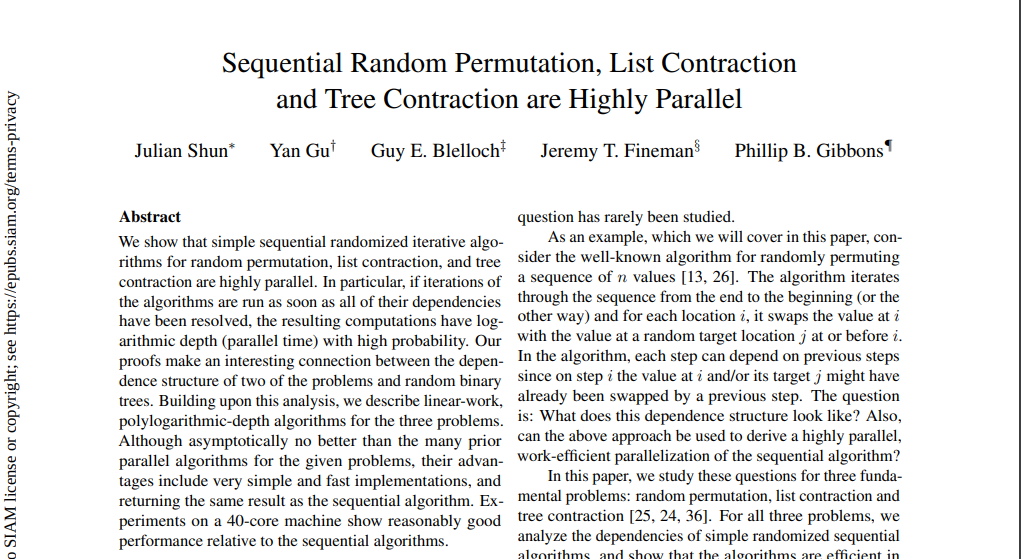
\includegraphics[width=0.60\textwidth]{julian-paper}
    \end{center}
    \caption{Shun et al. \cite{julian-parperm}}
  \end{figure}
\end{frame}

\begin{frame}{Parallel Knuth Shuffle}
  \begin{center}
    \Large{Main result: If we are able to detect if a step is
      \textit{ready} in constant time, then Knuth Shuffle can be
      run with \(\Theta(n)\) work and \(O(\log n)\) span.}
  \end{center}
\end{frame}

\begin{frame}{Deterministic Reservation}
  A framework by Blelloch et al. \cite{blelloch-detreserve} for developing
  parallel algorithms.
  \begin{itemize}
    \item Splits iteration into 2 phases: Reservation and Committing
    % \item Reserve decides what should be processed.
    % \item Commit carries out the processing.
    \item Primitive: \textsc{WriteMax(\(l, x\))} 
  \end{itemize}
\end{frame}
